We generated datasets from the LDA model for a range of parameters,
and tested the algorithms discussed in previous section on the
prediction task. For the LDA algorithm and our Projector algorithm, we
also have results for the recovery task. We experimented with $k$ from
$3$ to $30$, and in each case, a set of $\alpha$ and $\beta$ to cover
a wide range of $sig\_word$ and $sig\_topic$. See
figure~\ref{fig:predictResult} for the prediction results of the
algorithms on a representative set of datasets.
\begin{figure}[ht]
     \begin{center}

        \subfigure{

            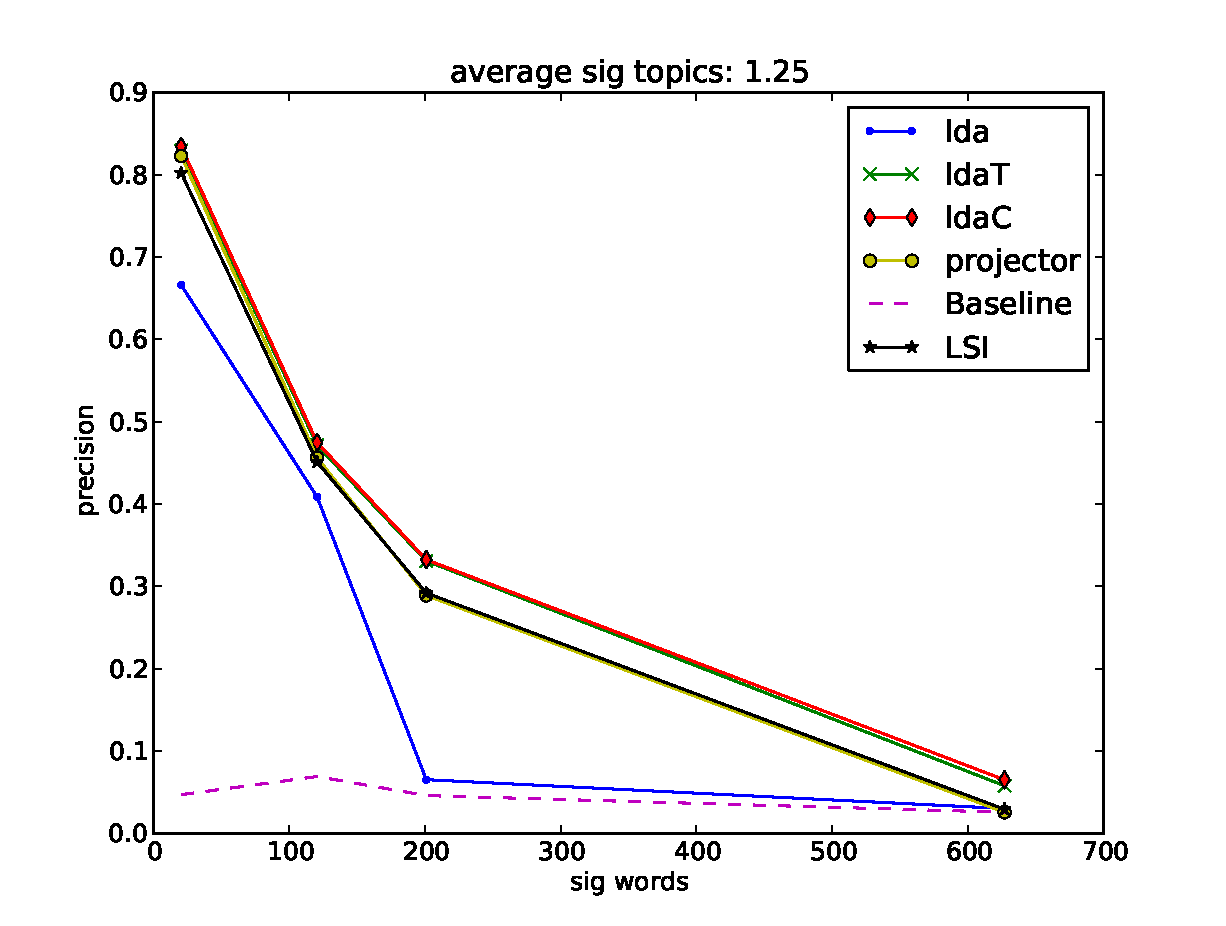
\includegraphics[width=0.45\textwidth]{k20a125.pdf}
        }
        \subfigure{

           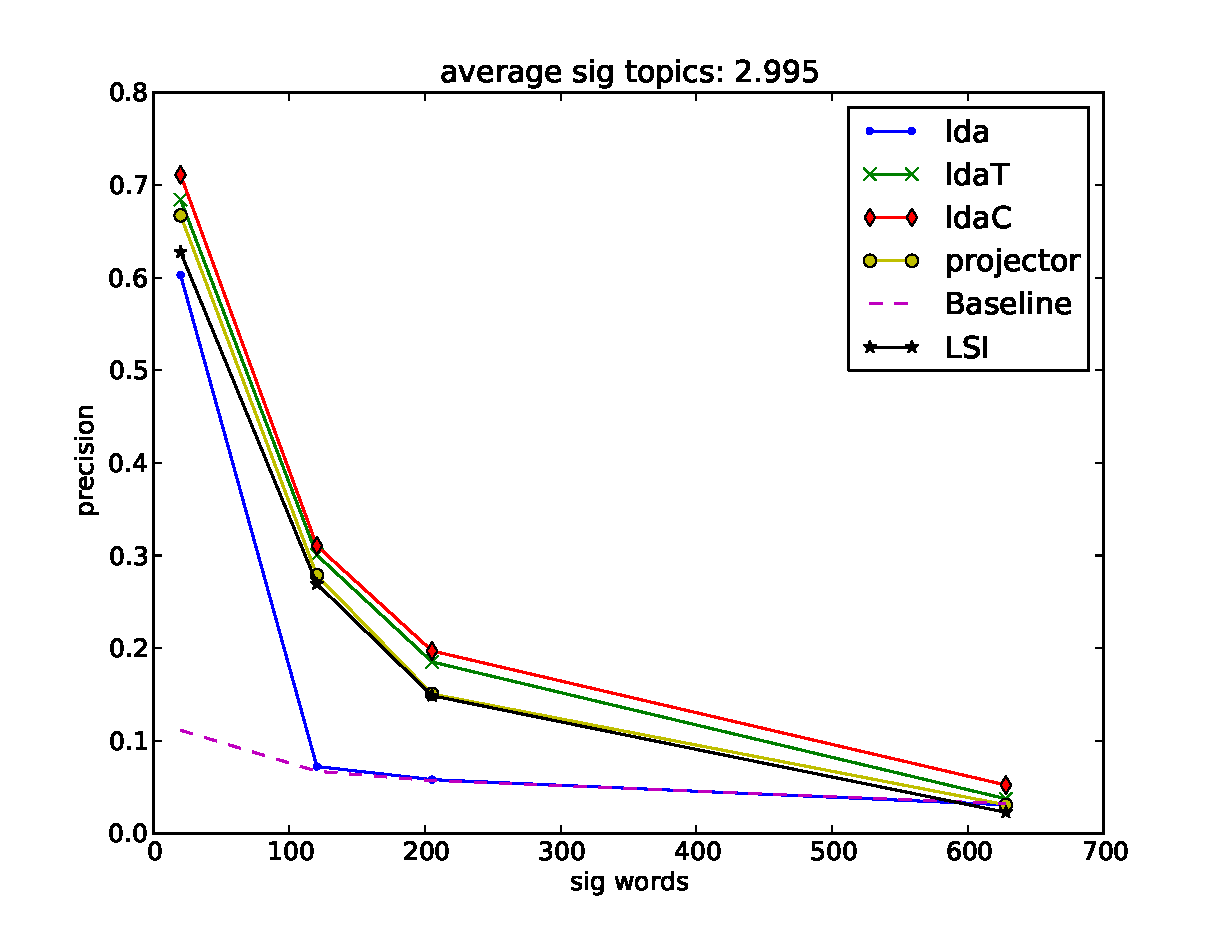
\includegraphics[width=0.45\textwidth]{k20a2995.pdf}
        }\\ 
        \subfigure{

            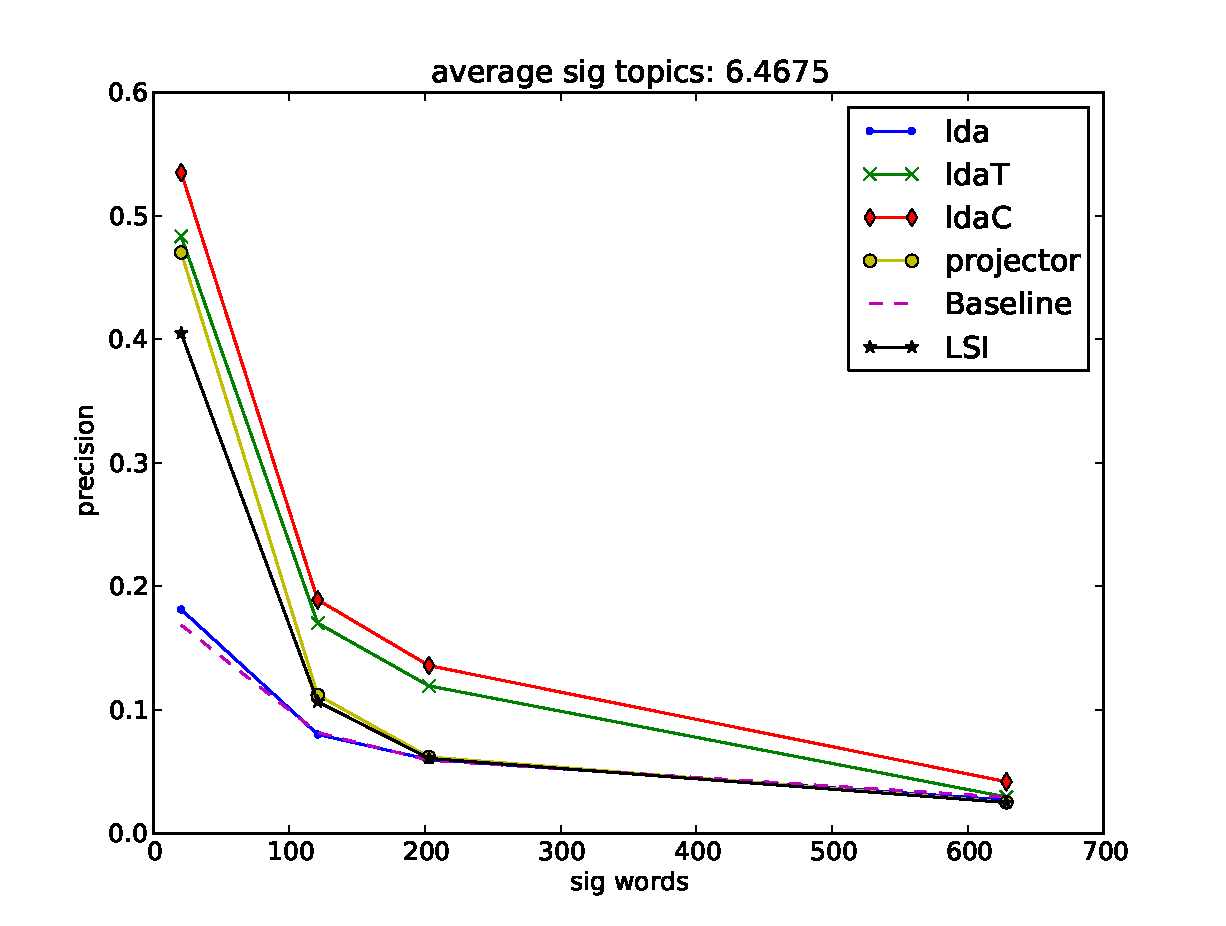
\includegraphics[width=0.45\textwidth]{k20a64675.pdf}
        }
        \subfigure{

            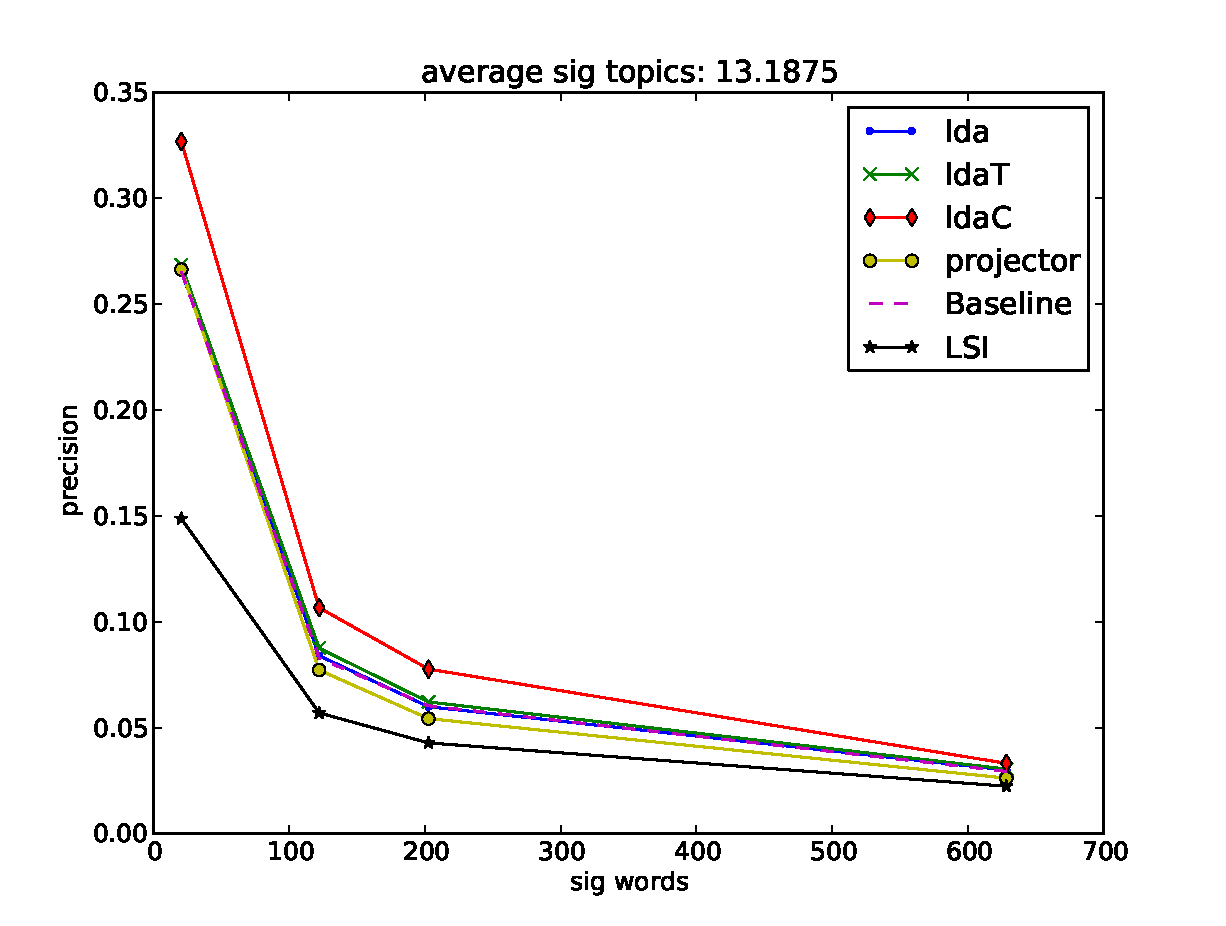
\includegraphics[width=0.45\textwidth]{k20a131875.pdf}
        }

    \end{center}
    \caption{Results of various algorithms on $16$ generated datasets, with $k=20, n=1000,m=1000,l=75$. Each subfigure has a fixed $sig\_topic$, the plots are result of the prediction task versus $sig\_word$}
   \label{fig:predictResult}
\end{figure}

\begin{table}[ht]
\begin{tabular}{|c|c|c|c|c|c|c|c|}
\hline 
 &Baseline &GibbsLda &LSI &PLSI &knn-25 &lda &projector \\
 \hline 
AP &0.14 &0.21 &0.24 &0.15 &0.25 &0.2 &0.21 \\
 \hline 
Cisi &0.09 &0.12 &0.09 &0.1 &0.14 &0.12 &0.1 \\
 \hline 
Cran &0.17 &0.21 &0.19 &0.17 &0.25 &0.23 &0.21 \\
 \hline 
Kos &0.21 &0.38 &0.26 &0.19 &0.38 &0.38 &0.3 \\
 \hline 
Med &0.08 &0.11 &0.16 &0.08 &0.17 &0.11 &0.16 \\
 \hline 
NIPS &0.64 &0.77 &0.47 &0.64 &0.75 &0.73 &0.57 \\
 \hline 

\end{tabular}
\caption{Experiment results on real datasets. We pick the result of the best among a few parameters for each algorithm. }
\label{tab:real}
\end{table}


Also see table~\ref{tab:real} for prediction results on real datasets.  There we see that
LDA is no longer dominated by LSI and Projector.  Still,  nearest neighbor's performance
dominates.  In the appendix, in table~\ref{tab:aptopics} we show the most popular
words in a sampling of topic vectors recovered by Projector in the AP dataset.

Typically, we saw the topic matching to correlate with prediction performance.
See figure~\ref{fig:size-matters} to see this result. 
